\begin{exercise}
      {ID-5d2ce9653ecf93debeaa5361ea778ea54f6de3dd}
      {Wolke}
  \newcommand{\zeichnung}
  {%
    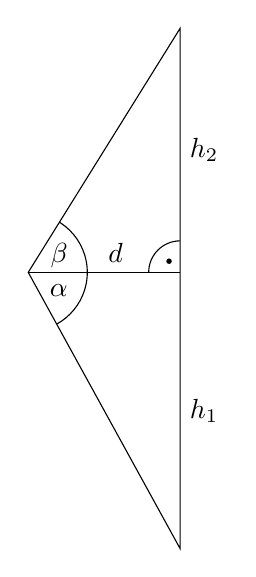
\begin{tikzpicture}[scale=0.05]
      \coordinate (A) at ( 0.000,  70.2);
      \coordinate (B) at (38.593,   0.0);
      \coordinate (C) at (38.593, 132.2);
      \coordinate (D) at (38.593,  70.2);
      \draw (A) -- (B) -- (C) -- cycle;
      \draw (A) -- (D);
      \path (B) -- node[right] {$h_{1}$} (D);
      \path (D) -- node[right] {$h_{2}$} (C);
      \path (A) -- node[above, pos=0.575] {$d$} (D);
      % alpha
      \begin{scope}
        \clip (A) -- (D) -- (B) -- cycle;
        \draw (A) circle[radius=15cm];
        \node at ([shift={(0, 70.2)}]329.4:9) {$\alpha$};
      \end{scope}
      % beta
      \begin{scope}
        \clip (A) -- (D) -- (C) -- cycle;
        \draw (A) circle[radius=15cm];
        \node at ([shift={(0, 70.2)}]29.05:9) {$\beta$};
      \end{scope}
      % rechter Winkel
      \begin{scope}
        \clip (A) -- (D) -- (C) -- cycle;
        \draw (D) circle[radius=8cm];
        \fill ([shift={(135:4cm)}]D) circle[radius=7mm];
      \end{scope}
    \end{tikzpicture}%
  }%
  \ifproblem\problem\par
    Ein Berghotel liegt \SI{70.2}{\metre} über dem Spiegel eines Sees.
    Vom Hotel aus sieht ein Beobachter eine Wolke unter dem Höhenwinkel
    \SI{58.1}{\degree}, ihr Spiegelbild im See unter dem Tiefenwinkel
    \SI{61.2}{\degree}. In welcher Höhe befindet sich die Wolke
    über dem See?
  \fi
  %\ifoutline\outline\par
  %\fi
  \ifoutcome\outcome\par
    \begin{center}
      \zeichnung
    \end{center}
    \begin{equation*}
      \begin{split}
        \tan\alpha=\frac{h_{1}}{d}
        &\quad\Rightarrow\quad
        d=\frac{h_{1}}{\tan\alpha}\\[2ex]
        \tan\beta=\frac{h_{2}}{d}
        &\quad\Rightarrow\quad
        h_{2}=d\cdot\tan\beta=h_{1}\cdot\frac{\tan\beta}{\tan\alpha}
      \end{split}
    \end{equation*}
  \fi
\end{exercise}
